\PassOptionsToPackage{unicode=true}{hyperref} % options for packages loaded elsewhere
\PassOptionsToPackage{hyphens}{url}
%
\documentclass[11pt,ignorenonframetext,]{beamer}
\usepackage{pgfpages}
\setbeamertemplate{caption}[numbered]
\setbeamertemplate{caption label separator}{: }
\setbeamercolor{caption name}{fg=normal text.fg}
\beamertemplatenavigationsymbolsempty
% Prevent slide breaks in the middle of a paragraph:
\widowpenalties 1 10000
\raggedbottom
\setbeamertemplate{part page}{
\centering
\begin{beamercolorbox}[sep=16pt,center]{part title}
  \usebeamerfont{part title}\insertpart\par
\end{beamercolorbox}
}
\setbeamertemplate{section page}{
\centering
\begin{beamercolorbox}[sep=12pt,center]{part title}
  \usebeamerfont{section title}\insertsection\par
\end{beamercolorbox}
}
\setbeamertemplate{subsection page}{
\centering
\begin{beamercolorbox}[sep=8pt,center]{part title}
  \usebeamerfont{subsection title}\insertsubsection\par
\end{beamercolorbox}
}
\AtBeginPart{
  \frame{\partpage}
}
\AtBeginSection{
  \ifbibliography
  \else
    \frame{\sectionpage}
  \fi
}
\AtBeginSubsection{
  \frame{\subsectionpage}
}
\usepackage{lmodern}
\usepackage{amssymb,amsmath}
\usepackage{ifxetex,ifluatex}
\usepackage{fixltx2e} % provides \textsubscript
\ifnum 0\ifxetex 1\fi\ifluatex 1\fi=0 % if pdftex
  \usepackage[T1]{fontenc}
  \usepackage[utf8]{inputenc}
  \usepackage{textcomp} % provides euro and other symbols
\else % if luatex or xelatex
  \usepackage{unicode-math}
  \defaultfontfeatures{Ligatures=TeX,Scale=MatchLowercase}
\fi
\usetheme[]{Montpellier}
\usecolortheme{beaver}
% use upquote if available, for straight quotes in verbatim environments
\IfFileExists{upquote.sty}{\usepackage{upquote}}{}
% use microtype if available
\IfFileExists{microtype.sty}{%
\usepackage[]{microtype}
\UseMicrotypeSet[protrusion]{basicmath} % disable protrusion for tt fonts
}{}
\IfFileExists{parskip.sty}{%
\usepackage{parskip}
}{% else
\setlength{\parindent}{0pt}
\setlength{\parskip}{6pt plus 2pt minus 1pt}
}
\usepackage{hyperref}
\hypersetup{
            pdftitle={Etude des effets des pésticides dans la production des vins de table},
            pdfauthor={A. Blanc, N. Gusarov, S. Picon},
            pdfborder={0 0 0},
            breaklinks=true}
\urlstyle{same}  % don't use monospace font for urls
\newif\ifbibliography
\usepackage{graphicx,grffile}
\makeatletter
\def\maxwidth{\ifdim\Gin@nat@width>\linewidth\linewidth\else\Gin@nat@width\fi}
\def\maxheight{\ifdim\Gin@nat@height>\textheight\textheight\else\Gin@nat@height\fi}
\makeatother
% Scale images if necessary, so that they will not overflow the page
% margins by default, and it is still possible to overwrite the defaults
% using explicit options in \includegraphics[width, height, ...]{}
\setkeys{Gin}{width=\maxwidth,height=\maxheight,keepaspectratio}
\setlength{\emergencystretch}{3em}  % prevent overfull lines
\providecommand{\tightlist}{%
  \setlength{\itemsep}{0pt}\setlength{\parskip}{0pt}}
\setcounter{secnumdepth}{0}

% set default figure placement to htbp
\makeatletter
\def\fps@figure{htbp}
\makeatother

\makeatletter
\setbeamertemplate{footline}{%
  \leavevmode%
  \hbox{%
  \begin{beamercolorbox}[wd=.333333\paperwidth,ht=2.25ex,dp=1ex,center]{author in head/foot}%
    \usebeamerfont{author in head/foot}\insertshortauthor
  \end{beamercolorbox}%
  \begin{beamercolorbox}[wd=.333333\paperwidth,ht=2.25ex,dp=1ex,center]{title in head/foot}%
    \usebeamerfont{institute in head/foot}\insertshortinstitute
  \end{beamercolorbox}%
  \begin{beamercolorbox}[wd=.333333\paperwidth,ht=2.25ex,dp=1ex,right]{date in head/foot}%
    \usebeamerfont{date in head/foot}\insertshortdate{}\hspace*{2em}
   %\insertframenumber{} / \inserttotalframenumber\hspace*{2ex} % old version
    \insertframenumber{} \hspace*{2ex} % new version without total frames
  \end{beamercolorbox}}%
  \vskip0pt%
}
\makeatother

\title{Etude des effets des pésticides dans la production des vins de table}
\providecommand{\subtitle}[1]{}
\subtitle{Analyse empirique des marchés}
\author{A. Blanc, N. Gusarov, S. Picon}
\providecommand{\institute}[1]{}
\institute{Université Grenoble Alpes}
\date{19/12/2019}

\begin{document}
\frame{\titlepage}

\hypertarget{introduction}{%
\section{Introduction}\label{introduction}}

\begin{frame}{Introduction}
\protect\hypertarget{introduction-1}{}

\center

\textbf{Quel est l'effet de l'utilisation des pesticides sur le marché des vins simples ?}

Dans cette étude, nous chercherons à étudier l'équilibre sur le marché
du vin.

\end{frame}

\begin{frame}{Plan de la présentation}
\protect\hypertarget{plan-de-la-presentation}{}

\begin{itemize}
\tightlist
\item
  Présentation de la problématique

  \begin{itemize}
  \tightlist
  \item
    Pesticides
  \item
    Marché du vin
  \end{itemize}
\item
  Le modèle théorique
\item
  Les données
\item
  Modélisation
\item
  Les résultats
\item
  Conclusion
\end{itemize}

\end{frame}

\hypertarget{les-pesticides}{%
\section{Les pesticides}\label{les-pesticides}}

\begin{frame}{Les pesticides}
\protect\hypertarget{les-pesticides-1}{}

\begin{itemize}
\tightlist
\item
  Présentation du problème des pésticides
\item
  Etat actuel
\item
  Comment baisser l'utilisation de pesticides
\end{itemize}

\end{frame}

\begin{frame}{Présentation du problème des pesticides}
\protect\hypertarget{presentation-du-probleme-des-pesticides}{}

\begin{itemize}
\tightlist
\item
  Source de nombreux débats sur la santé et l'environnement.
\item
  Le rôle actuel :

  \begin{itemize}
  \tightlist
  \item
    Moyen de protection contre les aléas climatiques ;
  \item
    Outil pour la réservation du rendement.
  \end{itemize}
\item
  Plusieurs mesures mises en places pour réduire leurs usages :

  \begin{itemize}
  \tightlist
  \item
    des interdiction des produits les plus toxiques ;
  \item
    l'instauration d'une taxe, payée par les agriculteurs (Butault et
    al, 2011).
  \end{itemize}
\item
  Malgres les efforts l'utilisation perdure :

  \begin{itemize}
  \tightlist
  \item
    Hausse des ventes de produits phytosanitaires ;
  \item
    Augmentation des doses utilisés (+12\% en 2014-2016) ;
  \end{itemize}
\end{itemize}

\end{frame}

\begin{frame}{Etat actuel}
\protect\hypertarget{etat-actuel}{}

Contrairement aux attentes des autorités aucune baisse de l'utilisation
de pesticides :

\begin{itemize}
\tightlist
\item
  Le nombre de doses unité augmente de 23\% entre 2008 et 2017 ;
\item
  Le nombre de substances actives utilisées a augmenté de 15\% entre
  2011 et 2017 ;
\item
  Une baisse des produits les plus dangereux de 6\%, en 2017 (Moghaddam
  et al, 2019) ;
\item
  Les grandes cultures (blés, etc\ldots{}) sont les premières
  utilisatrices de pesticides 67.4\% ;
\item
  Les vignes sont les deuxièmes 14.4\% (Butault et al, 2011).
\end{itemize}

\end{frame}

\begin{frame}{Comment baisser l'utilisation de pesticides}
\protect\hypertarget{comment-baisser-lutilisation-de-pesticides}{}

Les méthodes contemporaines visant à baisser l'utilisation des
pésticides sont :

\begin{itemize}
\tightlist
\item
  Le changement de mode de culture :

  \begin{itemize}
  \tightlist
  \item
    agriculture biologique ;
  \item
    agriculture raisonnée ;
  \end{itemize}
\item
  La diversification des cultures, ce qui est impossible pour la vigne
  (Moghaddam et al, 2019).
\end{itemize}

\end{frame}

\hypertarget{le-marche-du-vin-francais}{%
\section{Le marché du vin français}\label{le-marche-du-vin-francais}}

\begin{frame}{Le marché du vin français}
\protect\hypertarget{le-marche-du-vin-francais-1}{}

\begin{itemize}
\tightlist
\item
  Le vin français
\item
  Utilisation des pésticides dans la viticulture
\item
  Le problème d'heterogénéité
\item
  Les vins de table
\item
  Le marché des vins de table français
\end{itemize}

\end{frame}

\begin{frame}{Le vin français}
\protect\hypertarget{le-vin-francais}{}

France est un producteur de vin important :

\begin{itemize}
\tightlist
\item
  10\% surface de vigne mondiale ;
\item
  3\% de la surface agricole française est dediée au vin ;
\item
  16\% de la production mondiale ;
\item
  Le vin est la boisson alcoolisée la plus consommée en France ;
\item
  88\% des ventes de vins en France sont effectuées dans des grandes
  surfaces (CNIV, 2018).
\end{itemize}

La consommation de vins en France, tous types (FranceAgrimer, 2011) :

\begin{itemize}
\tightlist
\item
  55\% de vins rouges ;
\item
  16\% de vins blancs ;
\item
  29\% de vins rosés.
\end{itemize}

\end{frame}

\begin{frame}{Utilisation des pesticides dans la viticulture}
\protect\hypertarget{utilisation-des-pesticides-dans-la-viticulture}{}

La viticulture un type de culture gourmand en pesticides :

\begin{itemize}
\tightlist
\item
  14.4\% des produits phytosanitaires utilisés en France ;
\item
  2-ème culture utilisatrice de pesticides en France ;
\item
  Fortes disparités d'utilisation des pesticides entre les régions
  (Butault et al, 2011) ;
\item
  Les bassins viticoles Français utilisent en majorité des fongicides et
  des bactéricides sur la vigne ;
\item
  La champagne est la région la plus utilisatrice de pesticide avec un
  IFT de 21.4 en 2013 ;
\end{itemize}

\end{frame}

\begin{frame}{Le problème d'heterogénéité}
\protect\hypertarget{le-probleme-dheterogeneite}{}

Il existe une forte hétérogénéité entre les différents labels mais aussi
à l'intérieur de ces labels.

Les vins peuvent être divisés en 2 grandes classes suivant leurs prix
(Cembalo et al., 2014) :

\begin{itemize}
\tightlist
\item
  Les vins de qualité supérieure

  \begin{itemize}
  \tightlist
  \item
    limitation des quantités produites
  \item
    l'origine contrôlé
  \item
    une demande spécifique
  \end{itemize}
\item
  Les vins de qualité faible

  \begin{itemize}
  \tightlist
  \item
    hétérogènéité moins importante (Cembalo et al., 2014)
  \end{itemize}
\end{itemize}

\end{frame}

\begin{frame}{Les vins de table}
\protect\hypertarget{les-vins-de-table}{}

Les vins de tables sont des vins sans indication géographiques :

\begin{itemize}
\tightlist
\item
  hétérogènéité plus faible que pour les autre types ;
\item
  prix bas.
\end{itemize}

Nous traitons seulement des vins sans indication géographique :

\begin{itemize}
\tightlist
\item
  La situation sur ce marché influence l'utilisation des pesticides ;
\item
  Il existe une homogénéité presque parfaite dans les vins sans
  indication géographique (Cembalo et al, 2014).
\end{itemize}

\end{frame}

\begin{frame}{Le marché des vins de tables Français}
\protect\hypertarget{le-marche-des-vins-de-tables-francais}{}

Représente 10\% de la production (VIN \& SOCIETE, 2018)

\begin{itemize}
\tightlist
\item
  Hausse des transactions en 2011 :

  \begin{itemize}
  \tightlist
  \item
    Vins rouges : 29 \%
  \item
    Vins rosés : 13\%
  \item
    Vins blancs : 76\%
  \end{itemize}
\item
  Hausse des prix en 2011 :

  \begin{itemize}
  \tightlist
  \item
    Vins rouges : 12\%
  \item
    Vins rosés : 3\%
  \item
    Vins blancs : 13\%
  \end{itemize}
\end{itemize}

\end{frame}

\hypertarget{le-modele-theorique}{%
\section{Le Modèle théorique}\label{le-modele-theorique}}

\begin{frame}{Le Modèle théorique}
\protect\hypertarget{le-modele-theorique-1}{}

\begin{itemize}
\tightlist
\item
  Le rôle des pesticides dans la production du vin
\item
  Le rôle de la demande sur la production et l'offre en général
\item
  La formalisation et les équations
\end{itemize}

\end{frame}

\begin{frame}{Le rôle de la demande sur la production et l'offre en
génèral}
\protect\hypertarget{le-role-de-la-demande-sur-la-production-et-loffre-en-general}{}

\begin{itemize}
\tightlist
\item
  Nous supposons que sur le marché des vins simples la demande est
  unique pour toute la France.
\item
  La production de vin varie par département à cause de variations
  climatologiques
\item
  On observe l'équilibre sur le marché au niveau du pays. Ainsi, la
  quantité demandée = quantité offerte par l'ensemble des régions.
\item
  La demande de pesticides est inélastique au prix. Ainsi, la quantité
  de pesticides utilisée dépend seulement des intentions et des besoins
  des agriculteurs.
\end{itemize}

\end{frame}

\hypertarget{les-donnees}{%
\section{Les données}\label{les-donnees}}

\begin{frame}{Les données}
\protect\hypertarget{les-donnees-1}{}

\begin{itemize}
\tightlist
\item
  Souces des données
\item
  Déscription des données
\item
  Les variables choisi
\item
  Les variables utilisées pour notre modèle
\end{itemize}

\end{frame}

\begin{frame}{Sources des données :}
\protect\hypertarget{sources-des-donnees}{}

\begin{itemize}
\tightlist
\item
  Les données de ventes de pesticides par département (INERIS)
\item
  Les données sur les prix du vin (FranceAgrimer)
\item
  Les données sur la population (INSEE)
\item
  Les données sur la production de vin (SSM Finances Publiques)
\item
  Variation par département français (pour les régions produisant le
  vin)
\item
  Variation par année (2012 à 2016)
\end{itemize}

\end{frame}

\begin{frame}{Déscription des données :}
\protect\hypertarget{description-des-donnees}{}

\begin{itemize}
\tightlist
\item
  Toutes les variables varient par département et par année.
\item
  Le période temporelle comprise dans notre échantillon est de 2012 à
  2016.
\item
  Sélection des régions productrices de vin et utilisatrices de
  pesticides (69 départements).
\item
  Utilisation de l'echelle logarithmique afin de contracter la variance.
\end{itemize}

\end{frame}

\begin{frame}{Les variables utilisées pour notre modèle}
\protect\hypertarget{les-variables-utilisees-pour-notre-modele}{}

\begin{itemize}
\tightlist
\item
  Variables endogènes :

  \begin{itemize}
  \tightlist
  \item
    la quantité totale produite de vin rouge et blanc non IG par
    département (en hectolitres, en log),
  \item
    le prix moyen des vins rouges-blancs (idice, en log).
  \end{itemize}
\item
  Variables exogènes :

  \begin{itemize}
  \tightlist
  \item
    le revenu médian par département (en euros par personne par année,
    en log),
  \item
    la surface agricole destinée aux vins de table (en hectares, en
    log),
  \item
    la quantité des pesticides utilisés sur la vigne (indice, en log).
  \end{itemize}
\end{itemize}

\end{frame}

\hypertarget{letude-statistique}{%
\section{L'étude statistique}\label{letude-statistique}}

\begin{frame}{L'étude statistique}
\protect\hypertarget{letude-statistique-1}{}

\begin{itemize}
\tightlist
\item
  L'étude bivarié
\item
  L'étude de la variance
\item
  L'étude des types d'effets
\item
  L'analyse de la correlation
\item
  La transformation \textbf{within}
\end{itemize}

\end{frame}

\begin{frame}{Visualisatoin des interdependances}
\protect\hypertarget{visualisatoin-des-interdependances}{}

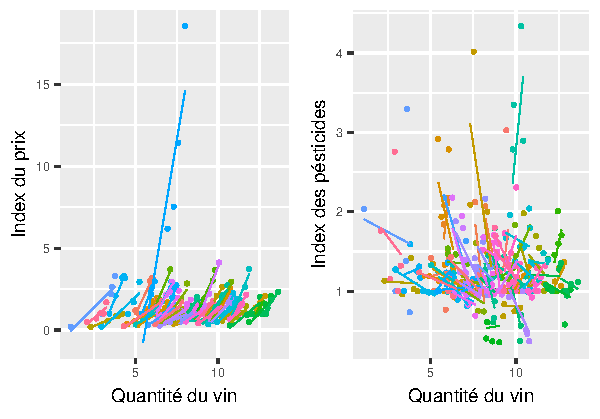
\includegraphics{Presentation_files/figure-beamer/unnamed-chunk-17-1.pdf}

\end{frame}

\begin{frame}{Visualisatoin des interdependances}
\protect\hypertarget{visualisatoin-des-interdependances-1}{}

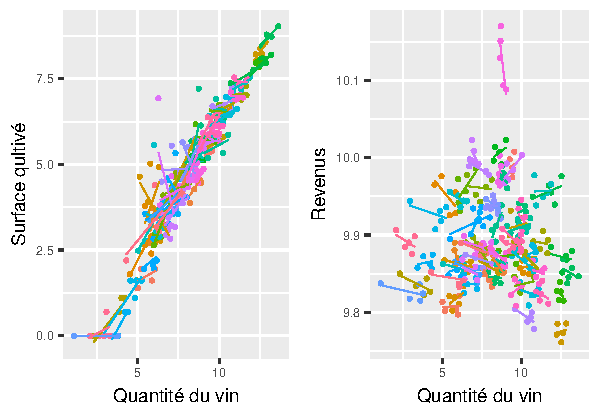
\includegraphics{Presentation_files/figure-beamer/unnamed-chunk-18-1.pdf}

\end{frame}

\begin{frame}{Etude de la variance}
\protect\hypertarget{etude-de-la-variance}{}

\tiny
\begin{table}[!htbp] \centering 
  \caption{Variance study}
\begin{tabular}{@{\extracolsep{5pt}} l|cccc} 
\\[-1.8ex]\hline 
\hline \\[-1.8ex] 
 & Mean & Overall & Between & Within \\ 
\hline \\[-1.8ex] 
Index prix & $0.175$ & $0.568$ & $0.368$ & $0.434$ \\ 
Index pesticides & $0.170$ & $0.333$ & $0.239$ & $0.234$ \\ 
Surface & $4.892$ & $1.986$ & $1.955$ & $0.410$ \\ 
Revenus & $9.891$ & $0.061$ & $0.061$ & $0.011$ \\ 
Temps & $3$ & $1.416$ & $0$ & $1.416$ \\ 
\hline \\[-1.8ex] 
\end{tabular} 
\end{table}

\normalsize

\tiny
\begin{table}[!htbp] \centering
  \caption{Chow pooling test}
\begin{tabular}{@{\extracolsep{5pt}} l|cc} 
\\[-1.8ex]\hline 
\hline \\[-1.8ex] 
 & Random & Fixed \\ 
\hline \\[-1.8ex] 
Index prix & $0.535$ & $0.533$ \\ 
Index pesticides & $0.485$ & $0.451$ \\ 
Surface & $0$ & $0.0001$ \\ 
Revenus & $0.297$ & $0.247$ \\ 
\hline \\[-1.8ex]
\end{tabular} 
\end{table}

\end{frame}

\begin{frame}{L'étude des types d'effets}
\protect\hypertarget{letude-des-types-deffets}{}

\tiny
\begin{table}[!htbp] \centering 
  \caption{Lagrange multiplier test, p-values}
\begin{tabular}{@{\extracolsep{5pt}} l|ccc} 
\\[-1.8ex]\hline 
\hline \\[-1.8ex] 
 & Individual & Time & Two-ways \\ 
\hline \\[-1.8ex] 
Index prix & $0$ & $0.169$ & $0$ \\ 
Index pesticides & $0$ & $0.222$ & $0$ \\ 
Surface & $0$ & $0.030$ & $0$ \\ 
Revenus & $0$ & $0.248$ & $0$ \\ 
\hline \\[-1.8ex] 
\end{tabular} 
\end{table}

\end{frame}

\begin{frame}{L'analyse de la correlation}
\protect\hypertarget{lanalyse-de-la-correlation}{}

\tiny
\begin{table}[!htbp] \centering
  \caption{Overall correlation}
\begin{tabular}{@{\extracolsep{5pt}} l|cccccc}
\\[-1.8ex]\hline
\hline \\[-1.8ex]
 & Quantité du vin & IP & Surface & Revenus & Index pésticides & Temps \\
\hline \\[-1.8ex]
Quantité du vin & $1$ & $0.154$ & $0.956$ & $-0.027$ & $-0.078$ & $-0.036$ \\      
IP & $0.154$ & $1$ & $0.045$ & $-0.037$ & $-0.127$ & $0.043$ \\
Surface & $0.956$ & $0.045$ & $1$ & $-0.057$ & $-0.060$ & $-0.064$ \\
Revenus & $-0.027$ & $-0.037$ & $-0.057$ & $1$ & $-0.052$ & $0.119$ \\
Index pésticides & $-0.078$ & $-0.127$ & $-0.060$ & $-0.052$ & $1$ & $0.291$ \\  
Temps & $-0.036$ & $0.043$ & $-0.064$ & $0.119$ & $0.291$ & $1$ \\
\hline \\[-1.8ex]
\end{tabular}
\end{table}

\tiny
\begin{table}[!htbp] \centering 
  \caption{Within transformation correlation}
\begin{tabular}{@{\extracolsep{5pt}} ccccccc} 
\\[-1.8ex]\hline 
\hline \\[-1.8ex] 
 & Quantité du vin & IP & Surface & Revenus & Index pésticides & Temps \\ 
\hline \\[-1.8ex] 
Quantité du vin & $1$ & $0.961$ & $0.366$ & $-0.160$ & $-0.228$ & $-0.199$ \\ 
IP & $0.961$ & $1$ & $0.289$ & $-0.009$ & $-0.127$ & $0.056$ \\ 
Surface & $0.366$ & $0.289$ & $1$ & $-0.166$ & $-0.191$ & $-0.310$ \\ 
Revenus & $-0.160$ & $-0.009$ & $-0.166$ & $1$ & $0.228$ & $0.652$ \\ 
Index pésticides & $-0.228$ & $-0.127$ & $-0.191$ & $0.228$ & $1$ & $0.414$ \\ 
Temps & $-0.199$ & $0.056$ & $-0.310$ & $0.652$ & $0.414$ & $1$ \\ 
\hline \\[-1.8ex] 
\end{tabular} 
\end{table}

\end{frame}

\begin{frame}{La transformation \textbf{within}}
\protect\hypertarget{la-transformation-within}{}

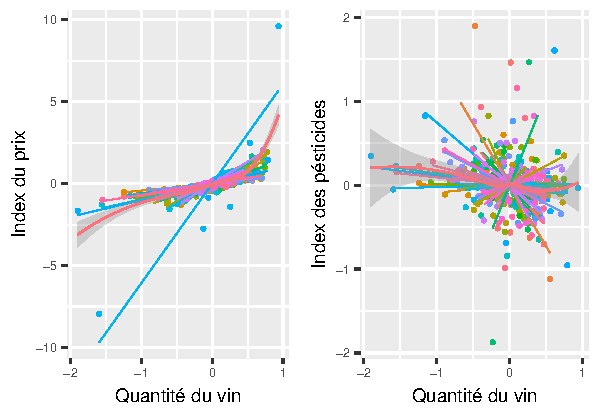
\includegraphics{Presentation_files/figure-beamer/unnamed-chunk-29-1.pdf}

\end{frame}

\begin{frame}{La transformation \textbf{within}}
\protect\hypertarget{la-transformation-within-1}{}

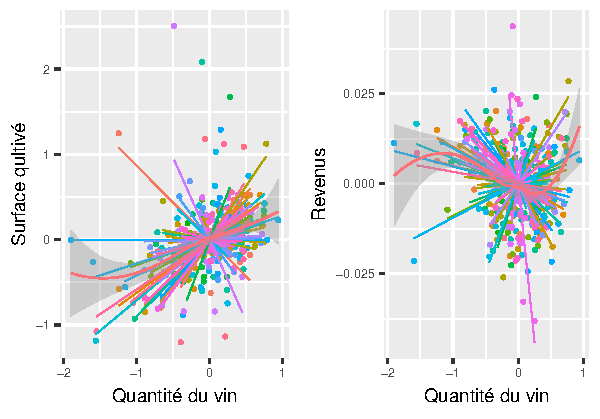
\includegraphics{Presentation_files/figure-beamer/unnamed-chunk-30-1.pdf}

\end{frame}

\hypertarget{modelisation}{%
\section{Modèlisation}\label{modelisation}}

\begin{frame}{Modèlisation}
\protect\hypertarget{modelisation-1}{}

\begin{itemize}
\tightlist
\item
  Presentation de la méthode
\item
  Les estimations

  \begin{itemize}
  \tightlist
  \item
    OLS, WLS et SUR
  \item
    2SLS, W2SLS, 3SLS et i3SLS
  \end{itemize}
\end{itemize}

\end{frame}

\begin{frame}{Presentation de la méthode}
\protect\hypertarget{presentation-de-la-methode}{}

\begin{itemize}
\tightlist
\item
  Explication de la méthode utilisée

  \begin{itemize}
  \tightlist
  \item
    Panel data

    \begin{itemize}
    \tightlist
    \item
      Within transforation
    \item
      Fixed effects
    \item
      Obtained slopes are averages for all population
    \end{itemize}
  \item
    AIDS model

    \begin{itemize}
    \tightlist
    \item
      Interdependent equations (simultaneity bias)
    \item
      3SLS estimator (that is identical to ILS estimator)
    \item
      It generates consistent estimates
    \item
      The distribution of the estimators are normally distributed only
      in large samples
    \item
      The estimator is (asymptotically) efficient
    \end{itemize}
  \end{itemize}
\item
  Limites du modèle

  \begin{itemize}
  \tightlist
  \item
    Faible representation des effets hetérogenes entre les régions (nous
    estimons seulemnt les effets moyens)
  \item
    Les interferences induites par l'heterogénéité
  \end{itemize}
\end{itemize}

\end{frame}

\begin{frame}{Résultats des estimation}
\protect\hypertarget{resultats-des-estimation}{}

\begin{itemize}
\tightlist
\item
  Les coefficients estimés avec leurs variance
\item
  L'efficience et comparaison des estimateurs
\item
  Etude des erreurs

  \begin{itemize}
  \tightlist
  \item
    La distribution des erreurs

    \begin{itemize}
    \tightlist
    \item
      La normalité
    \item
      Centrage sur 0
    \item
      Independance des variables explicatives
    \end{itemize}
  \item
    L'autocorrelation des résidus
  \item
    L'hétéroskedacité
  \end{itemize}
\end{itemize}

\end{frame}

\begin{frame}{Les résultats OLS, WLS et SUR}
\protect\hypertarget{les-resultats-ols-wls-et-sur}{}

\tiny

\begin{table}
\begin{center}
\begin{tabular}{l c c c }
\hline
 & OLS & WLS & SUR \\
\hline
Demande: ipi        & $0.93^{***}$  & $0.93^{***}$  & $0.93^{***}$  \\
                    & $(0.01)$      & $(0.01)$      & $(0.01)$      \\
Demande: ri         & $-5.75^{***}$ & $-5.75^{***}$ & $-2.00^{***}$ \\
                    & $(0.47)$      & $(0.47)$      & $(0.33)$      \\
Offre: ipi          & $0.90^{***}$  & $0.90^{***}$  & $0.92^{***}$  \\
                    & $(0.01)$      & $(0.01)$      & $(0.01)$      \\
Offre: si           & $0.08^{***}$  & $0.08^{***}$  & $0.02^{*}$    \\
                    & $(0.01)$      & $(0.01)$      & $(0.01)$      \\
Offre: iki          & $-0.17^{***}$ & $-0.17^{***}$ & $-0.05^{**}$  \\
                    & $(0.02)$      & $(0.02)$      & $(0.02)$      \\
\hline
Demande: R$^2$      & 0.95          & 0.95          & 0.94          \\
Offre: R$^2$        & 0.94          & 0.94          & 0.93          \\
Demande: Adj. R$^2$ & 0.95          & 0.95          & 0.94          \\
Offre: Adj. R$^2$   & 0.94          & 0.94          & 0.93          \\
Num. obs. (total)   & 690           & 690           & 690           \\
\hline
\multicolumn{4}{l}{\scriptsize{$^{***}p<0.001$, $^{**}p<0.01$, $^*p<0.05$}}
\end{tabular}
\caption{Statistical models}
\label{table : ols, wls and sur}
\end{center}
\end{table}
\tiny

\end{frame}

\begin{frame}{Independance des résidus}
\protect\hypertarget{independance-des-residus}{}

\tiny
\begin{table}[!htbp] \centering 
  \caption{Correlation des résidus} 
\begin{tabular}{@{\extracolsep{5pt}} ccccccc} 
\\[-1.8ex]\hline 
\hline \\[-1.8ex] 
 & OLS D & OLS O & WLS D & WLS O & SUR D & SUR O \\ 
\hline \\[-1.8ex] 
Vin & $0.232$ & $0.244$ & $0.232$ & $0.244$ & $0.273$ & $0.275$ \\ 
IP & $-0$ & $-0$ & $0$ & $-0$ & $0$ & $0$ \\ 
Surface & $0.271$ & $-0$ & $0.271$ & $0$ & $0.313$ & $0.236$ \\ 
Revenus & $0$ & $-0.480$ & $-0$ & $-0.480$ & $-0.393$ & $-0.542$ \\ 
Pesticides & $-0.308$ & $-0$ & $-0.308$ & $0$ & $-0.373$ & $-0.281$ \\
\hline \\[-1.8ex] 
\end{tabular} 
\end{table}

\end{frame}

\begin{frame}{L'autocorrelation et l'hétéroskedacité}
\protect\hypertarget{lautocorrelation-et-lheteroskedacite}{}

\tiny
\begin{table}[!htbp] \centering 
  \caption{Durbin-Watson test statistics}
\begin{tabular}{@{\extracolsep{5pt}} cccc} 
\\[-1.8ex]\hline
\hline \\[-1.8ex] 
 & OLS & WLS & SUR \\ 
\hline \\[-1.8ex] 
Equation de demande & $1.129$ & $1.129$ & $1.583$ \\ 
Equation d'offre & $1.062$ & $1.062$ & $1.549$ \\ 
\hline \\[-1.8ex]
\end{tabular} 
\end{table}

\tiny 
\begin{table}[!htbp] \centering 
  \caption{Bartlett heteroscedasticity test} 
\begin{tabular}{@{\extracolsep{5pt}} cccc} 
\\[-1.8ex]\hline 
\hline \\[-1.8ex] 
 & OLS & WLS & SUR \\ 
\hline \\[-1.8ex] 
Equation de demande & $0.828$ & $0.828$ & $1$ \\ 
Equation d'offre & $0.999$ & $0.999$ & $1$ \\ 
\hline \\[-1.8ex]
\end{tabular} 
\end{table}

\end{frame}

\begin{frame}{Le comportement des résidus}
\protect\hypertarget{le-comportement-des-residus}{}

\tiny
\begin{table}[!htbp] \centering 
  \caption{Shapiro-Wilk normality test}
\begin{tabular}{@{\extracolsep{5pt}} cccc} 
\\[-1.8ex]\hline 
\hline \\[-1.8ex] 
 & OLS & WLS & SUR \\ 
\hline \\[-1.8ex] 
Equation de demande & $0$ & $0$ & $0$ \\ 
Equation d'offre & $0.0003$ & $0.0003$ & $0$ \\ 
\hline \\[-1.8ex] 
\end{tabular} 
\end{table}

\end{frame}

\begin{frame}{Les PDF des résidus}
\protect\hypertarget{les-pdf-des-residus}{}

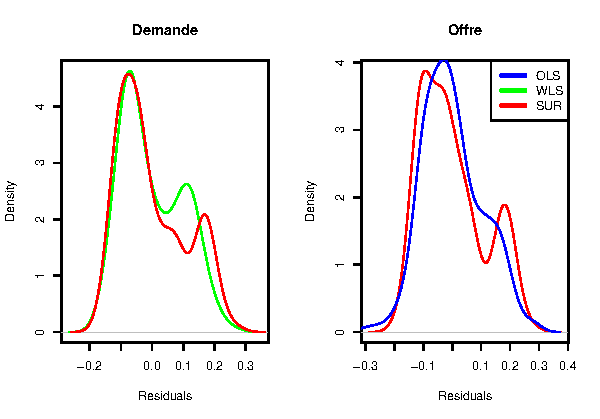
\includegraphics{Presentation_files/figure-beamer/unnamed-chunk-46-1.pdf}

\end{frame}

\begin{frame}{Les résidus contre la variable prédite}
\protect\hypertarget{les-residus-contre-la-variable-predite}{}

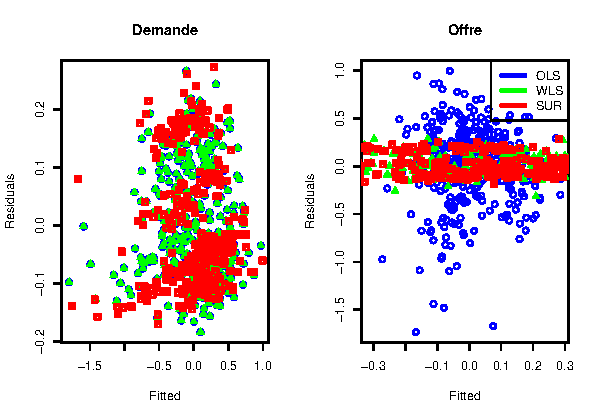
\includegraphics{Presentation_files/figure-beamer/unnamed-chunk-47-1.pdf}

\end{frame}

\begin{frame}{Les résultats 2SLS, W2SLS, 3SLS et i3SLS}
\protect\hypertarget{les-resultats-2sls-w2sls-3sls-et-i3sls}{}

\tiny

\begin{table}
\begin{center}
\begin{tabular}{l c c c c }
\hline
 & 2SLS & W2SLS & 3SLS & i3SLS \\
\hline
Demande: ipi        & $1.19^{***}$  & $1.19^{***}$  & $1.19^{***}$  & $1.19^{***}$  \\
                    & $(0.06)$      & $(0.06)$      & $(0.06)$      & $(0.06)$      \\
Demande: ri         & $-5.67^{***}$ & $-5.67^{***}$ & $-5.67^{***}$ & $-5.67^{***}$ \\
                    & $(0.71)$      & $(0.71)$      & $(0.71)$      & $(0.71)$      \\
Offre: ipi          & $-1.22$       & $-1.22$       & $-0.71$       & $-0.81$       \\
                    & $(1.97)$      & $(1.97)$      & $(1.96)$      & $(1.60)$      \\
Offre: si           & $0.70$        & $0.70$        & $0.46$        & $0.51$        \\
                    & $(0.59)$      & $(0.59)$      & $(0.58)$      & $(0.47)$      \\
Offre: iki          & $-0.46$       & $-0.46$       & $-0.73^{*}$   & $-0.68^{*}$   \\
                    & $(0.34)$      & $(0.34)$      & $(0.32)$      & $(0.26)$      \\
\hline
Demande: R$^2$      & 0.88          & 0.88          & 0.88          & 0.88          \\
Offre: R$^2$        & -3.37         & -3.37         & -1.60         & -1.90         \\
Demande: Adj. R$^2$ & 0.88          & 0.88          & 0.88          & 0.88          \\
Offre: Adj. R$^2$   & -3.40         & -3.40         & -1.62         & -1.92         \\
Num. obs. (total)   & 690           & 690           & 690           & 690           \\
\hline
\multicolumn{5}{l}{\scriptsize{$^{***}p<0.001$, $^{**}p<0.01$, $^*p<0.05$}}
\end{tabular}
\caption{Statistical models}
\label{table : 2sls, w2sls, 3sls and fiml}
\end{center}
\end{table}
\tiny

\end{frame}

\begin{frame}{Comparaison des modèles}
\protect\hypertarget{comparaison-des-modeles}{}

\tiny

\begin{table}[!htbp] \centering 
  \caption{Hausman 3SLS consistency test} 
  \label{} 
\begin{tabular}{@{\extracolsep{5pt}} ccc} 
\\[-1.8ex]\hline 
\hline \\[-1.8ex] 
 & Test & Resultats \\ 
\hline \\[-1.8ex] 
1 & 2SLS contre 3SLS & $0.350$ \\ 
2 & 2SLS contre i3SLS & $0.735$ \\ 
\hline \\[-1.8ex] 
\end{tabular} 
\end{table} 
\tiny

\tiny
\begin{table}[!htbp] \centering 
  \caption{Likelihood test} 
\begin{tabular}{@{\extracolsep{5pt}} cccccc} 
\\[-1.8ex]\hline 
\hline \\[-1.8ex] 
 & \#Df & LogLik & Df & Chisq & Pr(\textgreater Chisq) \\ 
\hline \\[-1.8ex] 
1 & $6$ & $-149.621$ & $-$ & $-$ & $-$ \\ 
2 & $8$ & $-65.614$ & $2$ & $168.013$ & $0$ \\ 
3 & $8$ & $-82.702$ & $0$ & $34.176$ & $0$ \\ 
\hline \\[-1.8ex] 
\end{tabular} 
\end{table}

\end{frame}

\begin{frame}{Le comportement des résidus}
\protect\hypertarget{le-comportement-des-residus-1}{}

\tiny
\begin{table}[!htbp] \centering 
  \caption{Shapiro-Wilk normality test}
\begin{tabular}{@{\extracolsep{5pt}} cccc} 
\\[-1.8ex]\hline 
\hline \\[-1.8ex] 
 & 2SLS & 3SLS & i3SLS \\ 
\hline \\[-1.8ex] 
Equation de demande & $0.00003$ & $0.00003$ & $0.00003$ \\ 
Equation d'offre & $0.00000$ & $0.00000$ & $0.00000$ \\ 
\hline \\[-1.8ex] 
\end{tabular} 
\end{table}

\tiny 
\begin{table}[!htbp] \centering 
  \caption{Bartlett heteroscedasticity test} 
\begin{tabular}{@{\extracolsep{5pt}} cccc} 
\\[-1.8ex]\hline 
\hline \\[-1.8ex]
 & 2SLS & 3SLS & i3SLS \\ 
\hline \\[-1.8ex] 
Equation de demande & $0.975$ & $0.975$ & $0.975$ \\ 
Equation d'offre & $0.0003$ & $0.002$ & $0.001$ \\ 
\hline \\[-1.8ex]
\end{tabular} 
\end{table}

\end{frame}

\begin{frame}{Les PDF des résidus}
\protect\hypertarget{les-pdf-des-residus-1}{}

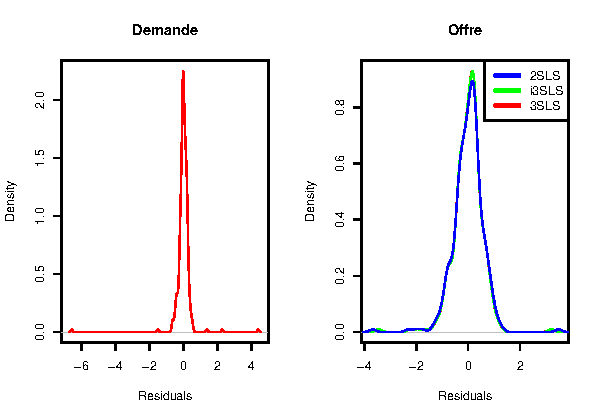
\includegraphics{Presentation_files/figure-beamer/unnamed-chunk-59-1.pdf}

\end{frame}

\begin{frame}{Les résidus contre la variable prédite}
\protect\hypertarget{les-residus-contre-la-variable-predite-1}{}

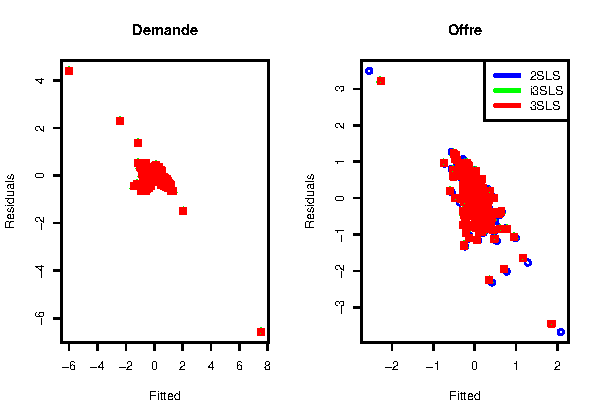
\includegraphics{Presentation_files/figure-beamer/unnamed-chunk-60-1.pdf}

\end{frame}

\begin{frame}{Les résidus et les prédictions pour i3SLS}
\protect\hypertarget{les-residus-et-les-predictions-pour-i3sls}{}

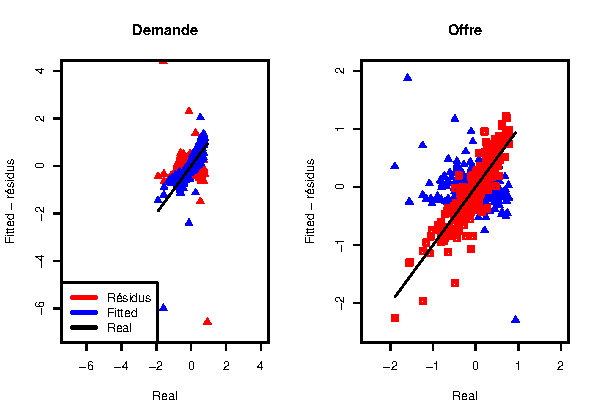
\includegraphics{Presentation_files/figure-beamer/unnamed-chunk-61-1.pdf}

\end{frame}

\begin{frame}{L'autocorrelation}
\protect\hypertarget{lautocorrelation}{}

\tiny
\begin{table}[!htbp] \centering 
  \caption{Durbin-Watson test statistics}
\begin{tabular}{@{\extracolsep{5pt}} cccc} 
\\[-1.8ex]\hline 
\hline \\[-1.8ex] 
 & 2SLS & 3SLS & i3SLS \\ 
\hline \\[-1.8ex] 
Equation de demande & $0.842$ & $0.842$ & $0.842$ \\ 
Equation d'offre & $0.643$ & $0.643$ & $0.643$ \\ 
\hline \\[-1.8ex]
\end{tabular}
\end{table}

\end{frame}

\begin{frame}{L'autocorrelation sur 2 dimentions pour i3SLS}
\protect\hypertarget{lautocorrelation-sur-2-dimentions-pour-i3sls}{}

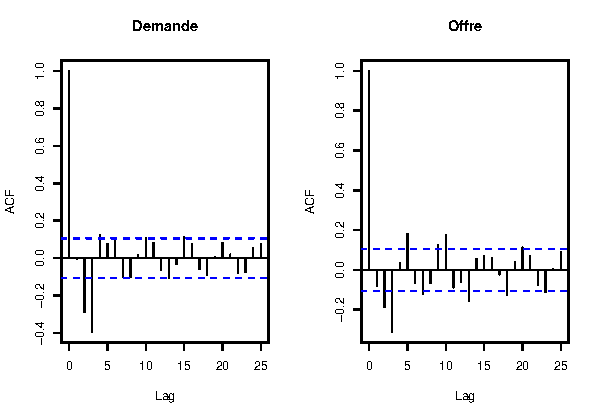
\includegraphics{Presentation_files/figure-beamer/unnamed-chunk-64-1.pdf}

\end{frame}

\begin{frame}{L'independance des résidus}
\protect\hypertarget{lindependance-des-residus}{}

\tiny
\begin{table}[!htbp] \centering
  \caption{Correlation des residus}
\begin{tabular}{@{\extracolsep{5pt}} ccccccc} 
\\[-1.8ex]\hline 
\hline \\[-1.8ex] 
 & 2SLS D & 2SLS O & 3SLS D & 3SLS O & i3SLS D & i3SLS O \\ 
\hline \\[-1.8ex]
Vin & $-0.561$ & $0.906$ & $-0.561$ & $0.898$ & $-0.561$ & $0.901$ \\ 
IP & $-0.746$ & $0.948$ & $-0.746$ & $0.938$ & $-0.746$ & $0.941$ \\ 
Surface & $-0.034$ & $0$ & $-0.034$ & $0.032$ & $-0.034$ & $0.024$ \\ 
Revenus & $0$ & $0$ & $-0$ & $0$ & $0$ & $-0$ \\ 
Pesticides & $-0.113$ & $0$ & $-0.113$ & $0.105$ & $-0.113$ & $0.080$ \\ 
\hline \\[-1.8ex]
\end{tabular} 
\end{table}

\end{frame}

\hypertarget{conclusions}{%
\section{Conclusions}\label{conclusions}}

\begin{frame}{Conclusions}
\protect\hypertarget{conclusions-1}{}

\begin{itemize}
\tightlist
\item
  Le marché du vin
\item
  Le rôle des pésticides\\
\item
  Validité
\end{itemize}

\end{frame}

\begin{frame}{Le marché du vin}
\protect\hypertarget{le-marche-du-vin}{}

\begin{itemize}
\tightlist
\item
  Un comportement inattendus

  \begin{itemize}
  \item
    Les effets de substitution contre les produits de la haute gamme
  \item
    Les effets négatives du revenu
  \item
  \end{itemize}
\end{itemize}

\end{frame}

\begin{frame}{Le rôle des pésticides}
\protect\hypertarget{le-role-des-pesticides}{}

\begin{itemize}
\tightlist
\item
  Confirmation des résultats des études précedentes

  \begin{itemize}
  \tightlist
  \item
    Utilisés pour réduire les pertes
  \end{itemize}
\end{itemize}

\end{frame}

\begin{frame}{Validité}
\protect\hypertarget{validite}{}

\begin{itemize}
\tightlist
\item
  Faible validité du modèle économétrique

  \begin{itemize}
  \tightlist
  \item
    Variables ommises
  \end{itemize}
\end{itemize}

\end{frame}

\begin{frame}{Bibliographie}
\protect\hypertarget{bibliographie}{}

\begin{itemize}
\tightlist
\item
  Cembalo L., Caracciolo F., \& Pomarici E. (2014). ``Drinking cheaply :
  the demand for basic wine in italy.'' \emph{Australian Journal of
  Agricultural and Resource Economics}, 58(3). 374-391.
\item
  Butault J-P., Delame N., Jacquet F. \& Zardet G. (2011).
  ``L'utilisation des pesticides en France: état des lieux et
  perspectives de réduction.'' \emph{Notes et études socio-économiques},
  35. 7-26
\item
  Pujol J. (2017). ``Apports des produits phytosanitaires en viticulture
  et climat : une analyse à partir des enquêtes pratiques culturales.''
  \emph{Agreste Les Dossiers}. 39. 3-25
\end{itemize}

\end{frame}

\end{document}
